\documentclass[a4paper,10pt]{report}
\usepackage{xunicode}
\usepackage{xltxtra}
\usepackage{color}
\usepackage{enumerate}
\usepackage[top=1.5cm, bottom=1.5cm, left=1.5cm, right=1.5cm]{geometry}
\usepackage{url}

\usepackage{minted}
\definecolor{frame_color}{gray}{0.70}
\addtolength\fboxsep{0.2cm}
\usemintedstyle{trac}
\newminted[code]{haskell}{xleftmargin=1cm, samepage=true}

\usepackage{fancyvrb}
%\DefineVerbatimEnvironment{code}{Verbatim}{frame=single, framerule=0.5mm, fontsize=\small, formatcom=\color{blue}}
%\DefineVerbatimEnvironment{example}{Verbatim}{}
\DefineShortVerb{\|}

\newcommand{\includeSource}[1]{
  \inputminted[frame=single, rulecolor=\color{frame_color}]{haskell}{#1}
}

\newcommand{\includeHaskell}[3]{
  The source code for this section is contained in \path{#1}.
  \begin{listing}[H]
  \inputminted[frame=single, rulecolor=\color{frame_color}]{haskell}{#1}
  \caption{#3}
  \label{lst:{#2}}
  \end{listing}
}

\title{Créatúr Tutorial}
\author{Amy de Buitl\'eir\\
        Email: amy@nualeargais.ie}

\begin{document}

\maketitle

\tableofcontents

\section{Overview of Créatúr}

Créatúr\footnote{\emph{Créatúr} (pronounced kray-toor) is an irish word 
meaning animal, creature, or unfortunate person.} 
is a software framework for automating experiments
with artificial life (ALife). 
It provides a daemon which ensures that each agent gets its turn 
to use the CPU. 
You can use other applications on the computer at the same time
without fear of interfering with experiments; they
will run normally (although perhaps more slowly).
Créatúr also provides a library of modules to help you implement your own 
ALife species.
Even if you aren't using the Créatúr framework, you may find some of these
modules useful.

\section{The main daemon loop}
\label{sec:daemon}

The daemon clock is a simple counter used to schedule events.
At each tick of the clock, the daemon

\begin{enumerate}
\item Reads the current list of agents, which are stored as separate files in
the current directory.
\item Queues the agents in random order.
\item Processes the queue, giving each agent an opportunity
to use the CPU by invoking a user-supplied function.
\item Increments the daemon clock.
\end {enumerate}

A different random order is used at each clock tick
so that no agent has an unfair advantage.
For example, if agents were always processed in the same order, 
agents near the end of the list might find that that the desirable mating
partners are already taken.

\section{Overview of the process}

The steps for using Créatúr to create and run an ALife experiment
are listed below.

\begin{enumerate}
\item Create one or more ALife species
\item Generate an initial population
\item Configure a daemon
\item Build and run the universe
\end {enumerate}

All examples discussed in this tutorial are available from
\url{https://github.com/mhwombat/creatur/archive/master.zip}.

\section{Example 1: A very simple species}
\label{sec:rock}

In this part of the tutorial, we create and run a universe
with a very simple species.
This will introduce you to the basics of the Créatúr framework.

\subsection{Create a species}
\label{sec:species1}

We'll only use one species in this example, and it will be a very simple 
species called |Rock|.
Rocks don't reproduce, so we don't need to worry about genetics.

A complete listing of the source code discussed here is provided on 
page \pageref{code:rock}.
We'll discuss the main points here.
The |DeriveGeneric| pragma activates support for generics
(available beginning with GHC 7.2 or the Haskell Platform 2012.4.0.0),
so we don't have to write functions to serialise and deserialise
the agents.

\begin{code}
{-# LANGUAGE DeriveGeneric #-}
\end{code} 

|Rock|s have a unique ID, and a counter. 
We will use the counter to demonstrate that the Créatúr
framework persists (``remembers'') the state of the rock
from one run to the next.

\begin{code}
data Rock = Rock String Int deriving (Show, Generic)
\end{code} 

All agents used in the Créatúr framework must be an instance of
|Serialize|, which ensures that they can be written to and read from a
database or file system.
Notice that we do not need to write |put| and |get| functions.
Deriving |Generic| instructs Haskell to generate them for us.

\begin{code}
instance Serialize Rock
\end{code} 

All species used in the Créatúr framework must be an instance of 
|ALife.Creatur.Agent|,
which requires us to implement two functions: |agentId| and |isAlive|.
The function |agentId| returns a unique identifier for this agent.
The function |isAlive| indicates whether the agent is currently alive
(if it is not alive, it would automatically be archived).
Since rocks never die, this function can simply return |True|.

\begin{code}
instance Agent Rock where
  agentId (Rock name _) = name
  isAlive _ = True
\end{code} 

Making |Rock| an instance of |ALife.Creatur.Database.Record|
allows us to store agents and retrieve them from the file system.
A record needs a unique identifier;
we can use |agentId| for this purpose.

\begin{code}
instance Record Rock where key = agentId
\end{code} 

Finally, we need to write the function that will be
invoked by the daemon when it is the agent's turn to use the CPU.
This function is passed as a configuration parameter to the daemon,
as will be seen in Section \ref{sec:daemon1}.
This example is quite simple;
it merely writes a message to the log file
and returns a new version of the rock, with an updated counter.
However, this is where your agents get a chance to eat, mate, 
and do whatever else they need to do.
We'll see a more typical implementation in Section
\ref{sec:bug}.

\begin{code}
run :: Rock -> StateT (SimpleUniverse a) IO Rock
run (Rock name k) = do
  writeToLog $ name ++ "'s turn. counter=" ++ show k 
  return $ Rock name (k+1)
\end{code}

The type signature of |run| is explained in Section \ref{sec:daemon1}.
The complete code listing is below.
\label{code:rock}
\includeSource{src/Tutorial/Example1/Rock.hs}



\subsection{Generate an initial population}
\label{sec:pop1}

We will create our first population in a directory called |Example1|.
In |main|, we initialise the |example1| directory, create two rocks,
and write them to the directory.

\includeSource{src/Tutorial/Example1/GeneratePopulation.hs}



The procedure for running this program will be described in Section 
\ref{sec:run1}.

\subsection{Configure a daemon}
\label{sec:daemon1}


The module \path{ALife.Creatur.Universe.Task} provides some tasks
that you can use with the daemon.
These tasks handle reading and writing agents,
which reduces the amount of code you need to write.
(It's also easy to write your own tasks, using those in 
\path{ALife.Creatur.Universe.Task} as a guide.)
The simplest task has the type signature:

\begin{code}
runNoninteractingAgents ∷ (Clock c, Logger l, Database d, Agent a, 
    Serialize a, Record a, a ~ DBRecord d) ⇒
  AgentProgram c l d n x a → StateT (Universe c l d n x a) IO ()
\end{code}

That signature looks complex, but essentially it means that if you
supply an |AgentProgram|, it will run it for you.
Your |AgentProgram| will run in a universe that implements
\path{ALife.Creatur.AgentNamer},
\path{ALife.Creatur.Clock}, and
\path{ALife.Creatur.Logger}.
So what type signature must your |AgentProgram| have?
Here's the definition.

\begin{code}
type AgentProgram c l d n x a = a → StateT (Universe c l d n x a) IO a
\end{code}

This is the signature for an agent that doesn't interact with other
agents.
The input parameter is the agent whose turn it is to use the CPU.
The program must return the agent (which may have been modified).
The universe will then automatically be updated with these changes.
We will use the |run| function in \path{Tutorial.Example1.Rock}
(discussed in Section \ref{sec:species1}) as our |AgentProgram|.
Its type signature is shown below.

\begin{code}
run :: Rock -> StateT (SimpleUniverse a) IO Rock
\end{code}

|SimpleUniverse a| provides the logging, clock, and agent naming
functionality we need, and satisfies |Universe c l d n x a|.
So the type signature of |run| is consistent with |AgentProgram|.
The program below configures and launches the daemon.

\includeSource{src/Tutorial/Example1/Daemon.hs}



\subsection{Build and run the example}
\label{sec:run1}


Here is the listing of |creatur-examples.cabal|.
\verbatiminput{creatur-examples.cabal}

\begin{enumerate}
\item Make sure you're in the directory containing |creatur-examples.cabal|.
\item Type |cabal install|.
\item Create the initial population by running |example1-init|.
\item Start the daemon with the command |sudo example1-daemon start|.
\item Stop the daemon with the command |sudo example1-daemon stop|.
(Stopping the daemon may take a few seconds.)
\end{enumerate}

Log messages are sent to |rocktopia/log/Rocktopia.log|.
Examine that file and notice that the counter is counting up for both rocks.
If you stop the daemon and restart it, it will pick up where it left off
\footnote{When the stop command is received, the daemon will attempt
to finish the processing for the current clock tick.
Depending on the processor speed and the number of agents in the population,
it may not finish before the hard kill which is issued three seconds later.
The database or file system is not updated until an agent's turn at the CPU 
is complete, so any partial results are discarded.
If the daemon terminates while an agent is running,
the effect is that the current agent, and all others after it in the queue,
miss their turn at the CPU.
However, even frequent restarting of the daemon
is unlikely to cause CPU starvation for any particular agent.
The random order in which agents are processed spreads the impact
over the population.}, preserving the value of the 
counter between runs.

A sample extract from the log file is shown below.
The first field is the system clock time.
The second field is the daemon clock time.
The third field is the log message.
Note that in clock tick |0|, |Rocky| gets to use the CPU before |Rocky|,
while in clock tick |3|, |Roxie| goes first.
This demonstrates the randomisation discussed in section \ref{sec:daemon}.

\begin{verbatim}
130121121233+0000       Starting
130121121233+0000       0       Rocky's counter is 42
130121121233+0000       0       Roxie's counter is 99
130121121233+0000       1       Rocky's counter is 43
130121121233+0000       1       Roxie's counter is 100
130121121233+0000       2       Roxie's counter is 101
130121121233+0000       2       Rocky's counter is 44
130121121233+0000       3       Roxie's counter is 102
130121121233+0000       3       Rocky's counter is 45
130121121234+0000       4       Rocky's counter is 46
130121121234+0000       4       Roxie's counter is 103
\end{verbatim}

\section{Recombination}
\label{sec:recombination}

When agents that reproduce, the offspring will inherit a mixture of
genetic information from both parents.
Here are two scenarios that could be used, although there are other
possibilities.

\begin{enumerate}
\item Your agents use \emph{asexual} reproduction.
Each agent has a \emph{single} sequence of genetic information.
When two agents mate, their genes are shuffled to produce
two \emph{new} sequences.
You can create two children from these sequences,
or discard one sequence and create a child with the remaining sequence.
\item Your agents use \emph{sexual} reproduction.
Each agent has \emph{two} sequences of genetic information.
When two agents mate, each agent contributes \emph{one}
sequence to the child.
A parent's two sequences are shuffled to produce two \emph{new}
sequences.
One of the sequences is discarded; the other sequence becomes
that parent's contribution to the child's genome.
The same process occurs with the other parent's genome.
The two sequences (one from each parent) are combined to create the 
child's genome.
This is analogous to the production of a \emph{gamete} (ovum or sperm) 
in biology.
\end{enumerate}

Both scenarios involve shuffling a pair of sequences to produce two new
pairs, and possibly discarding one of the sequences.
In addition, you may wish to allow occasional random mutations.
The Créatúr framework provides the 
several operations for this purpose, in the
\path{ALife.Creatur.Genetics.Recombination} package.
These operations can be applied (multiple times)
with specified probabilities
and combined in various ways.
Two common operations, \emph{crossover} and \emph{cut-and-splice},
are illustrated below.
In crossover, a single crossover point is chosen.
All data beyond that point is swapped between strings.
In cut-and-splice, two points are chosen, one on each string.
This generally results in two strings of unequal length.

\begin{figure}[hbtp]
 \centering
 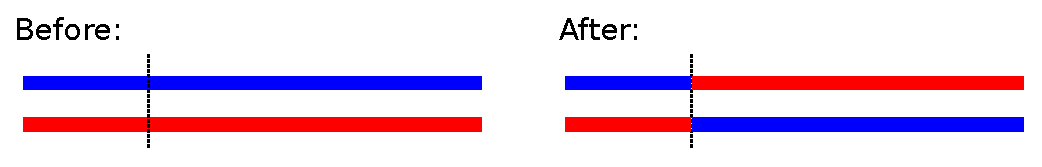
\includegraphics[scale=0.7,keepaspectratio=true]{./images/crossover.eps}
  \caption{Crossover}
  \label{fig:crossover}
\end{figure}

\begin{figure}[hbtp]
 \centering
 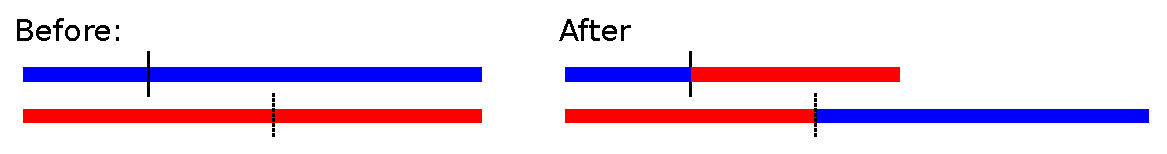
\includegraphics[scale=0.7,keepaspectratio=true]{./images/cut-and-splice.eps}
  \caption{Cut-and-splice}
  \label{fig:cut-and-splice}
\end{figure}

Here's a sample program that might be used to shuffle two
sequences of genetic material.

\label{code:recombination}
\begin{code}
    withProbability 0.1 randomCrossover (xs, ys) >>=
    withProbability 0.01 randomCutAndSplice >>=
    withProbability 0.001 mutatePairedLists >>=
    randomOneOfPair
\end{code} 

To understand how this program works,
let's walk through a simple example.
Suppose this program acted on the following pair of sequences:
|([A,A,A,A,A,A,A,A,A,A],[C,C,C,C,C,C,C,C,C,C])|.
The first line \emph{might} perform a simple crossover,
perhaps resulting in  |([A,A,A,A,A,A,A,C,C,C],[C,C,C,C,C,C,C,A,A,A])|.
The second line \emph{might} then perform a cut-and-splice, perhaps
resulting in |([A,A,A,A,C,A,A,A],[C,C,C,C,C,C,A,A,A,C,C,C])|.
The third line \emph{might} then mutate one or both sequences, perhaps
resulting in |([T,A,A,A,C,A,A,A],[C,C,C,C,C,C,A,A,C,C,C,C])|.
The numbers 0.1, 0.01, and 0.001 control the likelihood of each
of the three operations occurring.
After the first three operations, we have two new sequences.
In this example, we only want one of the sequences,
so the final line randomly chooses one.

To perform more than one crossover, the operation can simply be repeated
as shown below.

\begin{code}
    withProbability 0.1 randomCrossover (xs, ys) >>=
    withProbability 0.08 randomCrossover (xs, ys) >>=
    . . .
\end{code} 

Alternatively, we can choose the number of crossover operations at 
random. The function |repeatWithProbability| performs an operation a
random number of times, such that the probability of repeating the
operation |n| times is $p^n$.

\begin{code}
    repeatWithProbability 0.1 randomCrossover (xs, ys) >>=
    . . .
\end{code} 

Other recombination operators are also available.
Consult the documentation of \path{ALife.Creatur.Genetics.Recombination}
for more information.

\section{Example 2: Asexual reproduction}
\label{sec:plant}

In this part of the tutorial, we create a species with the
ability to reproduce asexually.

\subsection{Create a species}
\label{sec:species2}

The species used in this example is called |Plant|.
Each |Plant| has a unique ID, a flower colour,
an energy level, and some genetic information.
(A complete listing of the source code discussed here is provided on 
page \pageref{code:plant}.)

\begin{code}
data Plant = Plant
  { 
    plantName :: String,
    plantFlowerColour :: FlowerColour,
    plantEnergy :: Int,
    plantGenome :: [Bool]
  } deriving (Show, Generic)
\end{code} 

As with |Rock|s, the type |Plant| will be an instance of 
the |Serialize|, |Agent| and |Record|classes.
Our plants will stay alive until all of their energy is gone.

\begin{code}
instance Serialize Plant

instance Agent Plant where
  agentId = plantName
  isAlive plant = plantEnergy plant > 0

instance Record Plant where key = agentId
\end{code} 

We'll have a choice of flower colours.
\begin{code}
data FlowerColour = Red | Orange | Yellow | Violet | Blue
  deriving (Show, Eq, Generic, Enum, Bounded)
\end{code} 

In order for |Plant| to be an instance of |Serialize|,
any type that it uses must also be an instance.

\begin{code}
instance Serialize FlowerColour
\end{code} 

We need a way to encode the plant genes into DNA-like sequences that can
be shuffled, or even mutated, during reproduction.
We'll encode the genes as sequences of |Bool|s.
We could write our own coding scheme, but
the function |mkGrayCode| automatically generates one for us.
A Gray code maps values to codes in a way that guarantees that the codes
for two consecutive values will differ by only one bit. This feature
is useful for encoding genes because the result
of a crossover operation will be similar to the inputs. 
This helps to
ensure that offspring are similar to their parents, as any radical
changes from one generation to the next are the result of mutation
alone.

\begin{code}
colourCode :: Code FlowerColour Bool
colourCode = mkGrayCode [Red .. Blue]
\end{code} 

To support reproduction, we need a way to build a plant from its genome.
If a mutation occurs, the resulting sequence of |Bool|s may not
be a valid code for a colour, in which case the call to |decodeNext|
will return |Nothing|.
Similarly, if a cut-and-splice operation occurs,
the child could end up with a short sequence that has no colour gene.
In this example, we'll use a default colour of |Red|.
(Alternatively, we could treat the mutation as non-viable,
and not create the offspring.
We'll see an example of that in Section {sec:bug}.)
All plants start life with an energy of |10|.
        
\begin{code}
buildPlant :: String -> [Bool] -> Plant
buildPlant name g = Plant name colour 10 g
  where colour = fromMaybe Red c
        (c, _) = decodeNext colourCode g
\end{code} 

We need a way to mate two plants and produce some offspring.
We can do this by implementing the |Reproductive| class in 
\path{ALife.Creatur.Genetics.Reproduction.Asexual}.
This class requires us to implement the following:
\begin{enumerate}
\item A type called |Base|, which specifies the type used to encode
genes for this species. Recall that we've used |Bool|s for this purpose.
\item A method called |recombine| which shuffles (and maybe mutates) the
 parent's genes to produce the offspring.
\item A method called |build| which creates the offspring.
We can use the |buildPlant| method that we've already created,
but we need to wrap it in a |Maybe| to satisfy the type signature of
|build|.
\end {enumerate}

\begin{code}
instance Reproductive Plant where
  type Base Plant = Bool
  recombine a b = 
    withProbability 0.1 randomCrossover (plantGenome a, plantGenome b) >>=
    withProbability 0.01 randomCutAndSplice >>=
    withProbability 0.001 mutatePairedLists >>=
    randomOneOfPair
  build name g = Just $ buildPlant name g
\end{code} 

The implementation for |recombine| uses the sample recombination
program discussed on page \pageref{code:recombination}.
Next, we write the function |run|, 
which is invoked when it is the agent's turn to use the CPU.
Because our plants need to interact in order to mate,
when we write the daemon (in Section \ref{sec:daemon2}) we will use
|runInteractingAgents| instead of |runNoninteractingAgents|.
This requires a different type signature for |run| than we used for
rocks.
The type signature we need is

\begin{code}
type AgentsProgram c l d n x a = 
  [a] → StateT (Universe c l d n x a) IO [a]
\end{code} 

The input parameter is a list of agents. 
The first agent in the list is the agent whose turn it is to use the 
CPU.
The rest of the list contains agents it could interact with.
(We only need to use the first two elements of this list.)
Finally, the program must return a list of agents that it has modified.

The function |run| ``mates'' two plants and takes away one unit of energy 
to represent the energy cost of reproduction
(otherwise the plants would live forever).

\begin{code}
run :: [Plant] -> StateT (SimpleUniverse Plant) IO [Plant]
run (me:other:_) = do
  name <- genName
  (Just baby) <- liftIO $ evalRandIO (makeOffspring me other name)
  writeToLog $ 
    plantName me ++ " and " ++ plantName other ++
      " gave birth to " ++ name ++ ", with " ++ 
       show (plantFlowerColour baby) ++ " flowers"
  return [other, baby]
run x = return x -- need two agents to mate
\end{code}

The complete code listing is below.
\label{code:plant}
\includeSource{src/Tutorial/Example2/Plant.hs}



\subsection{Generate an initial population}
\label{sec:pop2}

We will create the next population in a directory called |example2|.
In |main|, we initialise the |example2| directory, create three 
|Plant|s, and write them to the directory.
The initial population only contains plants with red, yellow, 
or violet flowers.
Eventually, plants with orange or blue flowers might appear, but only
as the result of mutation.

\includeSource{src/Tutorial/Example2/GeneratePopulation.hs}



\subsection{Configure a daemon}
\label{sec:daemon2}

The program below configures and launches the daemon.

\includeSource{src/Tutorial/Example2/Daemon.hs}



\subsection{Build and run the example}
\label{sec:run2}

\begin{enumerate}
\item Make sure you're in the directory containing |creatur-examples.cabal|.
\item Type |cabal install| (if you haven't already done so).
\item Create the initial population by running |example2-init|.
\item Start/stop/restart the daemon with the command
\UndefineShortVerb{\|}
\DefineShortVerb{\+}
+sudo example2-daemon start|stop|restart+.
\UndefineShortVerb{\+}
\DefineShortVerb{\|}
(Stopping the daemon may take a few seconds.)
\end{enumerate}

Log messages are sent to |example2/log/Example2.log|.

A sample extract from the log file is shown below.
To conserve space, the timestamps have been omitted.
From this, you can see that the first mating (between |Rose| and |Sunny|)
occurs at time 0.
The offspring, |Example2_1|, gets its first CPU turn at time 1.

\begin{verbatim}
Starting
0       Vi and Rose gave birth to Example2_1, with Red flowers
0       Rose and Vi gave birth to Example2_2, with Violet flowers
0       Sunny and Rose gave birth to Example2_3, with Red flowers
1       Example2_1 and Sunny gave birth to Example2_4, with Yellow flowers
1       Rose and Vi gave birth to Example2_5, with Violet flowers
1       Example2_3 and Example2_2 gave birth to Example2_6, with Red flowers
1       Example2_2 and Sunny gave birth to Example2_7, with Violet flowers
1       Vi and Example2_7 gave birth to Example2_8, with Violet flowers
1       Sunny and Example2_8 gave birth to Example2_9, with Yellow flowers
2       Example2_4 and Rose gave birth to Example2_10, with Yellow flowers
2       Example2_7 and Example2_6 gave birth to Example2_11, with Violet flowers
2       Example2_6 and Rose gave birth to Example2_12, with Red flowers
2       Example2_5 and Example2_10 gave birth to Example2_13, with Violet flowers
2       Example2_3 and Example2_7 gave birth to Example2_14, with Red flowers
2       Example2_8 and Example2_14 gave birth to Example2_15, with Red flowers
2       Rose and Example2_14 gave birth to Example2_16, with Red flowers
2       Sunny and Example2_12 gave birth to Example2_17, with Yellow flowers
2       Vi and Example2_5 gave birth to Example2_18, with Violet flowers
\end{verbatim}

\section{Example 3: Sexual reproduction}
\label{sec:bug}

In this part of the tutorial, we create a species with the
ability to reproduce sexually.

\subsection{Create a species}
\label{sec:species3}

We create a type to represent the |Bug| species.
Each bug has a unique ID, a colour, sex, an energy level,
and a sequence of genetic information.

\begin{code}
data Bug = Bug
  { 
    bugName :: String,
    bugColour :: BugColour,
    bugSex :: Sex,
    bugEnergy :: Int,
    bugGenome :: ([Bool],[Bool])
  } deriving (Show, Generic)

instance Serialize Bug
\end{code} 

We make |Bug| implement the |Agent| 
and |Record| classes.
Our bugs will stay alive until their energy reaches zero.

\begin{code}
instance Agent Bug where
  agentId = bugName
  isAlive bug = bugEnergy bug > 0

instance Record Bug where key = agentId
\end{code} 

We create the genes for colour and sex.

\begin{code}
data BugColour = Green | Purple deriving (Show, Eq, Generic)
instance Serialize BugColour

data Sex = Male | Female deriving (Show, Eq, Generic)
instance Serialize Sex

colourCode :: Code BugColour Bool
colourCode = mkGrayCode [Green, Purple]

sexCode :: Code Sex Bool
sexCode = mkGrayCode [Male, Female]
\end{code} 

Because our bugs will reproduce \emph{sexually}, there's an extra step for
determining their characteristics based on their genome,
a step that was not necessary for plants.
Agents that reproduce sexually have \emph{two} sets of genes, 
one inherited from each parent.
These genes may not be identical,
so we need a function that determines the resulting colour of the bug
from its genes.
Let's make green \emph{dominant}, and purple \emph{recessive}.
This means that a bug with one green gene will be green,
no matter what the other gene is.
The only way that a bug can be purple is if both colour genes are purple.

\begin{code}
instance PairedGene BugColour where
  express Green _       = Green
  express _ Green       = Green
  express Purple Purple = Purple
\end{code} 

We need a similar function that determines the actual sex of the bug.
A bug with two |Female| genes is female, a bug with at least one 
|Male| gene is male.
(This is loosely based on the XY-chromosome system used by
humans and some other animals.)

\begin{code}
instance PairedGene Sex where
  express Male _        = Male
  express _ Male        = Male
  express Female Female = Female
\end{code} 

To support reproduction, we need a way to build a bug from its genome.
If a mutation occurs, the resulting sequence of |Bool|s may not
be a valid code for a colour, in which case the call to |decodeNext|
will return |Nothing|.

All bugs start life with 10 units of energy.
        
\begin{code}
buildBug :: String -> ([Bool], [Bool]) -> Bug
buildBug name g = Bug name colour sex 10 g
  where (s, g') = decodeAndExpress sexCode g
        (c, _) = decodeAndExpress colourCode g'
        sex = fromMaybe Female s
        colour = fromMaybe Green c
\end{code} 

Next, we need a way to mate two bugs and produce some offspring.
We can do this by implementing the |Reproductive| class in 
\path{ALife.Creatur.Genetics.Reproduction.Sexual}.
This class requires us to implement the following:
\begin{enumerate}
\item A type called |Base|, which specifies the type used to encode
genes for this species. Recall that we've used |Bool|s for this purpose.
\item A method called |produceGamete| which shuffles (and maybe mutates)
the two sequences of genes from one parent, 
and then produces a \emph{single} sequence that will become part of the
child's genome.
(This is analogous to creating either a single sperm or ova.)
\item A method called |build| which creates the offspring.
We can use the |buildBug| method that we've already created,
but we need to wrap it in a |Maybe| to satisfy the type signature of
|build|.
\end {enumerate}

\begin{code}
instance Reproductive Bug where
  type Base Bug = Bool
  produceGamete a = 
    repeatWithProbability 0.1 randomCrossover (bugGenome a) >>=
    withProbability 0.01 randomCutAndSplice >>=
    withProbability 0.001 mutatePairedLists >>=
    randomOneOfPair
  build name g = Just $ buildBug name g
\end{code} 

Although the implementation of |produceGamete| is similar to that
of |recombine| for the |Plant| class, 
these two functions have different uses.
Asexual reproduction uses |recombine| to mix the genetic
information from two parents;
the resulting sequence becomes the entire genome of the child.
Sexual reproduction uses |produceGamete| to mix the genetic information
from \emph{one} parent;
the resulting sequence becomes \emph{half} of the genome of the child.
The other half of the child's genome comes from the other parent,
also generated using |produceGamete|.

|runBug| is invoked when it is the agent's turn to use the CPU.
It triggers mating.
Just being alive costs energy, so we take away one
unit of energy.

\begin{code}
runBug :: Bug -> StateT (SimpleUniverse Bug) IO Bug
runBug bug = do
  writeToLog $ 
    bugName bug ++ " just woke up. Energy=" ++ show (bugEnergy bug)
  bug2 <- maybeMate bug
  let bug3 = bug2{ bugEnergy = bugEnergy bug2 - 1}
  if isAlive bug3
    then
      writeToLog $ 
        bugName bug3 ++ " is going back to sleep. Energy=" 
          ++ show (bugEnergy bug3)
    else writeToLog $ bugName bug ++ " is dead"
  return bug3
\end{code} 

Let's let the females initiate mating.
If this bug is female,
another bug is randomly selected as a potential mate.

\begin{code}
maybeMate :: Bug -> StateT (SimpleUniverse Bug) IO Bug
maybeMate bug =
  if bugSex bug == Female
    then do
      xs <- agentIds
      let otherIds = filter (bugName bug /=) xs
      otherId <- fromList $ zip otherIds (repeat (1 % 1))
      writeToLog $ bugName bug ++ " sees " ++ otherId
      withAgent (tryToMate bug) otherId
      return bug
    else return bug
\end{code} 

If the potential mate is male, then mating occurs.

\begin{code}
tryToMate :: Bug -> Bug -> StateT (SimpleUniverse Bug) IO Bug
tryToMate bug otherBug =
  if bugSex otherBug == Male
    then do
      writeToLog $ bugName bug ++ " mated with " ++ bugName otherBug ++ "."
      name <- genName
      (Just baby) <- liftIO $ evalRandIO (makeOffspring bug otherBug name)
      writeToLog $ 
        bugName bug ++ " and " ++ bugName otherBug ++
          " gave birth to " ++ name ++ ", a " ++ 
          show (bugColour baby) ++ " " ++ show (bugSex baby) ++ " bug"
      addAgent baby
      return otherBug
    else do
      writeToLog $ 
        bugName bug ++ " is not interested in " ++ bugName otherBug
          ++ "."
      return otherBug
\end{code}

\includeSource{src/Tutorial/Example3/Bug.hs}



\subsection{Generate an initial population}
\label{sec:pop3}

We will create the next population in a directory called |Example3|.
In |main|, we initialise the |example3| directory, create three Bugs,
and write them to the directory.
The bugs in the initial population will each have two identical
sequences of genetic material.

\includeSource{src/Tutorial/Example3/GeneratePopulation.hs}



\subsection{Configure a daemon}
\label{sec:daemon3}

The program below configures and launches the daemon.

\includeSource{src/Tutorial/Example3/Daemon.hs}



\subsection{Build and run the example}
\label{sec:run3}

\begin{enumerate}
\item Make sure you're in the directory containing |creatur-examples.cabal|.
\item Type |cabal install| (if you haven't already done so).
\item Create the initial population by running |example3-init|.
\item Start/stop/restart the daemon with the command
\UndefineShortVerb{\|}
\DefineShortVerb{\+}
+sudo example3-daemon start|stop|restart+.
\UndefineShortVerb{\+}
\DefineShortVerb{\|}
(Stopping the daemon may take a few seconds.)
\end{enumerate}

Log messages are sent to |example3/log/Example3.log|.

A sample extract from the log file is shown below.

\begin{verbatim}
130121134119+0000       Starting
130121134119+0000       0       Zelda just woke up. Energy=10
130121134119+0000       0       Zelda sees Mel
130121134119+0000       0       Zelda mated with Mel.
130121134119+0000       0       Zelda and Mel gave birth to Example3_1, a Green Male bug
130121134119+0000       0       Zelda is going back to sleep. Energy=9
130121134119+0000       0       Mel just woke up. Energy=10
130121134119+0000       0       Mel is going back to sleep. Energy=9
130121134119+0000       0       Betty just woke up. Energy=10
130121134119+0000       0       Betty sees Bugsy
130121134119+0000       0       Betty mated with Bugsy.
130121134119+0000       0       Betty and Bugsy gave birth to Example3_2, a Green Male bug
130121134119+0000       0       Betty is going back to sleep. Energy=9
130121134119+0000       0       Bugsy just woke up. Energy=10
130121134119+0000       0       Bugsy is going back to sleep. Energy=9
130121134119+0000       1       Mel just woke up. Energy=9
130121134119+0000       1       Mel is going back to sleep. Energy=8
130121134119+0000       1       Zelda just woke up. Energy=9
130121134119+0000       1       Zelda sees Example3_1
130121134119+0000       1       Zelda mated with Example3_1.
130121134119+0000       1       Zelda and Example3_1 gave birth to Example3_3, a Green Male bug
130121134119+0000       1       Zelda is going back to sleep. Energy=8
130121134119+0000       1       Betty just woke up. Energy=9
130121134119+0000       1       Betty sees Zelda
130121134119+0000       1       Betty is not interested in Zelda.
130121134119+0000       1       Betty is going back to sleep. Energy=8
130121134119+0000       1       Example3_1 just woke up. Energy=10
130121134119+0000       1       Example3_1 is going back to sleep. Energy=9
130121134119+0000       1       Example3_2 just woke up. Energy=10
130121134119+0000       1       Example3_2 is going back to sleep. Energy=9
130121134119+0000       1       Bugsy just woke up. Energy=9
130121134119+0000       1       Bugsy is going back to sleep. Energy=8
130121134120+0000       2       Example3_1 just woke up. Energy=9
130121134120+0000       2       Example3_1 is going back to sleep. Energy=8
130121134120+0000       2       Bugsy just woke up. Energy=8
130121134120+0000       2       Bugsy is going back to sleep. Energy=7
\end{verbatim}

\section{Example 4: Working with multiple species}
\label{sec:multiple}

In this part of the tutorial, we a universe with multiple species,
where each species is a different Haskell type.

\subsection{Create a species}
\label{sec:species4}

We can re-use the implementation of |Bug| from Section \ref{sec:bug},
but without the |run| method.
All agents will use the |run| method in \path{Tutorial.Example4.Martian}.

The complete code listing is below.
\includeSource{src/Tutorial/Example4/Rock.hs}


We can re-use the implementation of |Plant| from Section \ref{sec:plant},
with a few changes.
The code that implements mating has been moved into a custom
|tryMating| function.
Again, we can drop the |run| method because
all agents will use the |run| method in \path{Tutorial.Example4.Martian}.

The complete code listing is below.
\includeSource{src/Tutorial/Example4/Plant.hs}


We can re-use the implementation of |Bug| from Section \ref{sec:bug},
with a few changes.
The code that implements mating has been moved into a custom
|tryMating| function.
And again we can drop the |run| method.

The complete code listing is below.
\includeSource{src/Tutorial/Example4/Bug.hs}



\subsection{Generate an initial population}
\label{sec:pop4}

We will create the next population in a directory called |Example4|.
In |main|, we initialise the |example4| directory, create some rocks,
bugs, and plants, and then write them to the directory.

\includeSource{src/Tutorial/Example4/GeneratePopulation.hs}



\subsection{Configure a daemon}
\label{sec:daemon4}

The daemon implementation should be familiar by now.
\includeSource{src/Tutorial/Example4/Daemon.hs}





\subsection{Build and run the example}
\label{sec:run4}

\begin{enumerate}
\item Make sure you're in the directory containing |creatur-examples.cabal|.
\item Type |cabal install| (if you haven't already done so).
\item Create the initial population by running |example4-init|.
\item Start/stop/restart the daemon with the command
\UndefineShortVerb{\|}
\DefineShortVerb{\+}
+sudo example4-daemon start|stop|restart+.
\UndefineShortVerb{\+}
\DefineShortVerb{\|}
(Stopping the daemon may take a few seconds.)
\end{enumerate}

Log messages are sent to |example4/log/Example4.log|.

\section{TO DO}
\begin{enumerate}
\item Explain that if you don't want the child to be immediately mature,
you could have it be a field in the mother's implementation.

\item Show how to collect statistics.

\item Show how to keep agents and logs in a database rather than as separate
files. I'm thinking of providing an "agent interface" to MongoDB and any
ODBC-compliant DB.

\item Show how to get a list of agents meeting certain criteria 
(e.g. all agents within a certain distance of a particular agent).
This will require a different DB.

\item Show how to add other state data to the universe (in addition to
the clock, logger, agent namer, and database).
\end{enumerate}

\end{document}
